\documentclass[border=1pt]{standalone}
\usepackage[dvipsnames]{xcolor}
\usepackage{tikz}                       % Graphen und kommutative Diagramme
\usetikzlibrary{patterns}               % Um schraffierte Formen in der tikzpicture-Umgebung zu zeichnen.
\newcommand{\ul}[1]{\underline{\smash{#1}}}

\begin{document}

\centering
\begin{minipage}{.4\textwidth}
\centering
\resizebox{!}{4.5cm}{
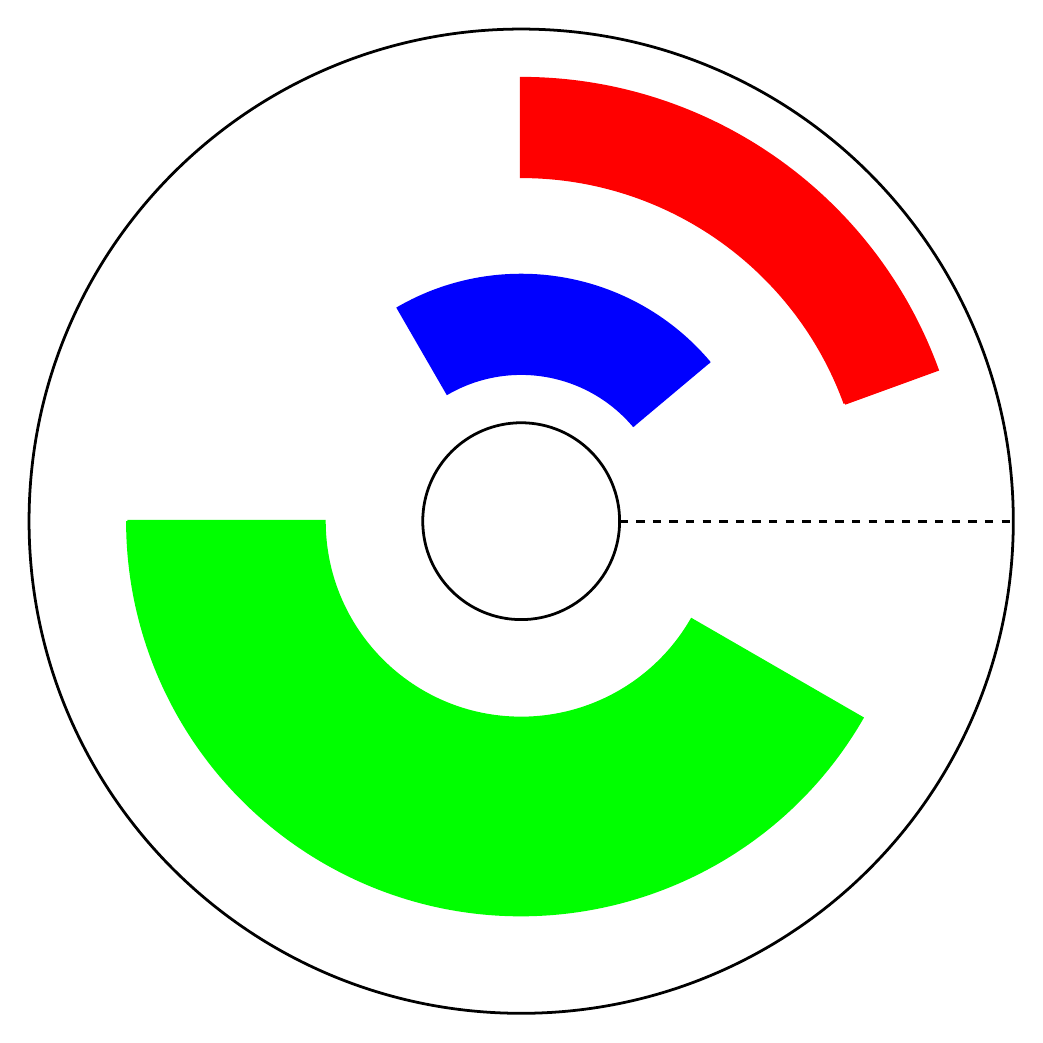
\begin{tikzpicture}[x=1.25cm, y=1.25cm, line width=1pt]
    % draw inner and outer circles
    \draw[color=black] (0, 0) circle (1);
    \draw[color=black] (0, 0) circle (5);
    
    % draw 0 line
    \draw[color=black, dashed] (0 : 1) -- (0 : 5); 
    
    % draw shaded slit box
    \filldraw[color = red] 
      (20 : 3.5) -- (20 : 4.5) arc [radius = 4.5, start angle = 20, delta angle = 70] 
	       -- (90 : 3.5) arc [radius = 3.5, start angle = 90, delta angle = -70];
    \filldraw[color = blue]
      (40 : 2.5) -- (40 : 2.5) arc [radius = 2.5, start angle = 40, delta angle = 80] 
	       -- (120 : 1.5) arc [radius = 1.5, start angle = 120, delta angle = -80];
    \filldraw[color = green]
        (180 : 4) -- (180 : 2) arc [radius = 2, start angle = 180, delta angle = 150] 
	       -- (330 : 4) arc [radius = 4, start angle = 330, delta angle = -150];
\end{tikzpicture}
}
\end{minipage}

\centering
\begin{minipage}{.4\textwidth}
\centering
\resizebox{!}{4.5cm}{
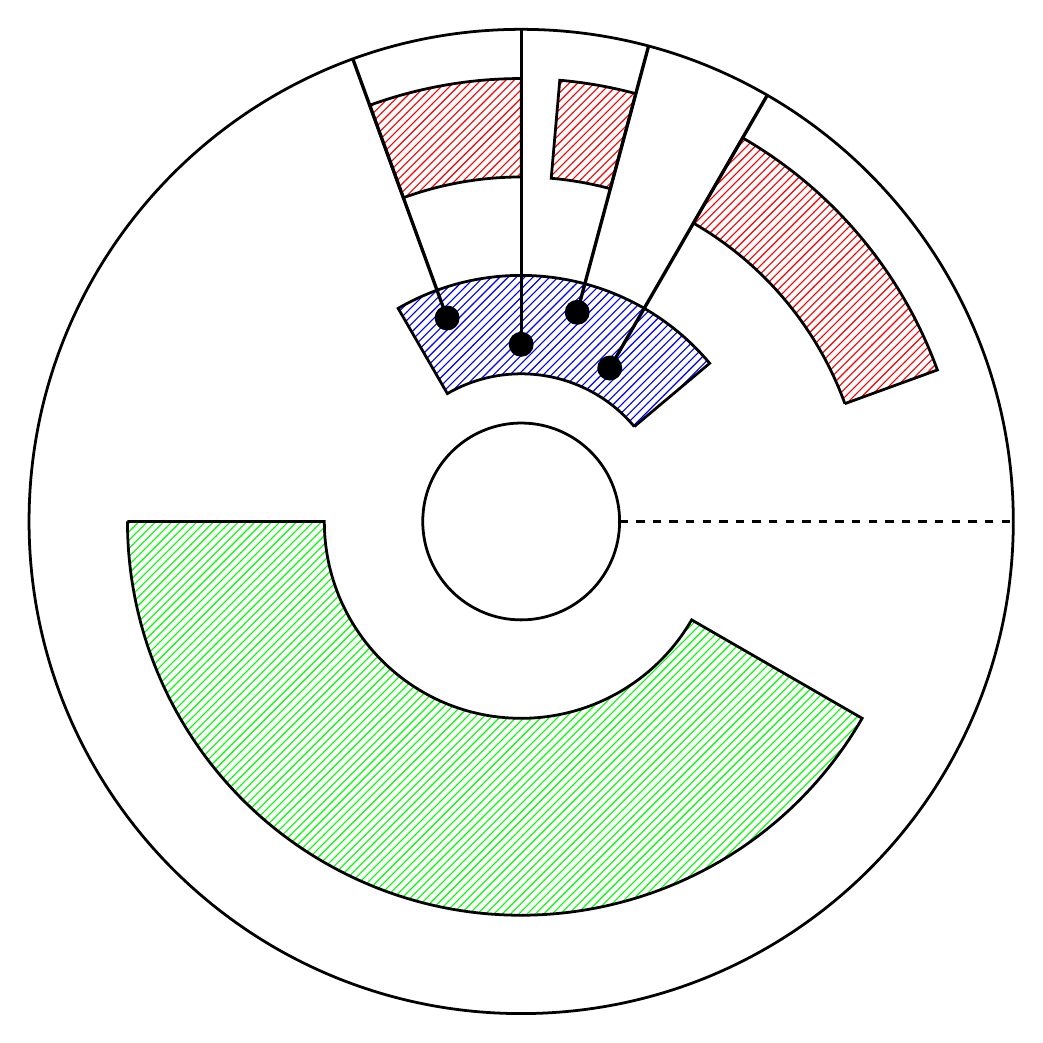
\begin{tikzpicture}[x=1.25cm, y=1.25cm, line width=1pt]
    % draw inner and outer circles
    \draw[color=black] (0, 0) circle (1);
    \draw[color=black] (0, 0) circle (5);
    
    % draw 0 line
    \draw[color=black, dashed] (0 : 1) -- (0 : 5); 
    
    % draw shaded slit box
    \filldraw[pattern=north east lines, pattern color=red] 
      (90 : 3.5) -- (90 : 4.5) arc [radius = 4.5, start angle = 90, delta angle = 20] 
	       -- (110 : 3.5) arc [radius = 3.5, start angle = 110, delta angle = -20];
    \filldraw[pattern=north east lines, pattern color=red] 
      (20 : 3.5) -- (20 : 4.5) arc [radius = 4.5, start angle = 20, delta angle = 40] 
	       -- (60 : 3.5) arc [radius = 3.5, start angle = 60, delta angle = -40];
    \filldraw[pattern=north east lines, pattern color=red] 
      (75 : 3.5) -- (75 : 4.5) arc [radius = 4.5, start angle = 75, delta angle = 10] 
	       -- (85 : 3.5) arc [radius = 3.5, start angle = 85, delta angle = -10];
    \filldraw[pattern=north east lines, pattern color=blue] 
      (40 : 1.5) -- (40 : 2.5) arc [radius = 2.5, start angle = 40, delta angle = 80] 
	       -- (120 : 1.5) arc [radius = 1.5, start angle = 120, delta angle = -80];
    \filldraw[pattern=north east lines, pattern color=green] 
      (180 : 4) -- (180 : 2) arc [radius = 2, start angle = 180, delta angle = 150] 
	       -- (330 : 4) arc [radius = 4, start angle = 330, delta angle = -150];
	       
     % draw slits
     \draw[color=black, line width=1.2pt] (60 : 5) -- (60 : 1.8);
     \filldraw[color = black, fill = black] (60 : 1.8) circle (4pt);

     \draw[color=black, line width=1.2pt] (90 : 5) -- (90 : 1.8);
     \filldraw[color = black, fill = black] (90 : 1.8) circle (4pt);
     
     \draw[color=black, line width=1.2pt] (110 : 5) -- (110 : 2.2);
     \filldraw[color = black, fill = black] (110 : 2.2) circle (4pt);
     
     \draw[color=black, line width=1.2pt] (75 : 5) -- (75 : 2.2);
     \filldraw[color = black, fill = black] (75 : 2.2) circle (4pt);
     
\end{tikzpicture}
}
\end{minipage}


\end{document}
